\lecture{Finite state methods in NLP}{finstatemeth}

\section{Finite State Automata}

\begin{frame}

	\begin{center}
		\Huge \insertsection
	\end{center}

\end{frame}


\begin{frame}

	\frametitle{\insertsection}
	
	\begin{enumerate}
		\item Finite State Recognizers and Generators
		\begin{enumerate}
			\item Basics and simple machines
			\item Finite State Automata
		\end{enumerate}
		\item Deterministic and Non-deterministic Automata
		\item Implementing FSA in Prolog
		\begin{enumerate}
			\item Defining FSA in Prolog
			\item A Recognizer and Generator in Prolog with no jumps
			\item A Recognizer and Generator in Prolog with jumping arcs
		\end{enumerate}
		\item Finite State Methods in Computational Linguistics and NLP
	\end{enumerate}

\end{frame}

\subsection{Finite State Recognizers and Generators}

\begin{frame}

	\frametitle{\insertsection}
	\framesubtitle{\insertsubsection}
	
	\begin{itemize}
		\item Finite State Automata are used in morphology, phonology, text to speech, and data mining.
		\item They are simple and well understood mathematically.
		\item They are easy to implement and implementations are usually very efficient.
		\item With all simplicity FSA are restricted in what they are able to do.
		\item There is not a finite state solution for every NLP problem.
	\end{itemize}

\end{frame}

\begin{frame}

	\frametitle{\insertsection}
	\framesubtitle{\insertsubsection}
	
	\begin{itemize}
		\item A \textbf{finite state generator} is a simple computing machine that outputs a sequence of symbols.
		\item FSG has a finite number of different states (obviously it has).
		\item It starts in some start state and then tries to reach a final state by making transitions from one state to another. Every time it makes such a transition it \textbf{emits} a symbol.
		\item It cannot stop until it reaches a final state.
		\item FSG only know the state it is currently in, and cannot look ahead at the states that come and also doesn't have any memory of the states it has been.
	\end{itemize}
	
\end{frame}


\begin{frame}

	\frametitle{\insertsection}
	\framesubtitle{\insertsubsection}
	
	\begin{itemize}
		\item Finite state generators can be thought of as directed graphs.
		\item In fact finite state generators are usually drawn as directed graphs.
	\end{itemize}

\end{frame}


\begin{frame}

	\frametitle{\insertsection}
	\framesubtitle{\insertsubsection}

	
	\only<1>{\begin{figure}
		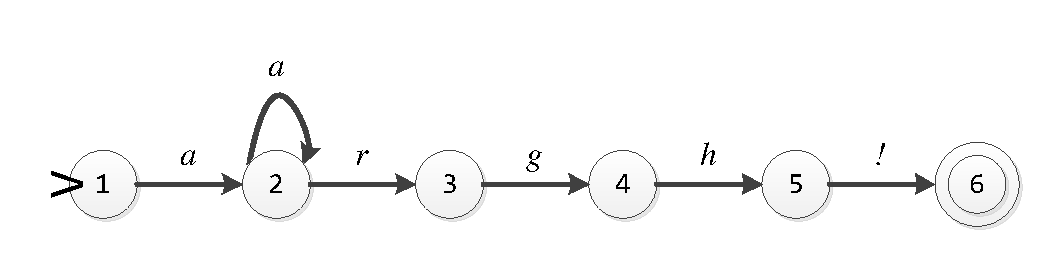
\includegraphics[scale=0.8]{screaming_machine}
	\end{figure}}

	\only<2->{\begin{figure}
			
\includegraphics[scale=0.85]{frustration}
	\end{figure}}
	
\end{frame}


\begin{frame}

	\frametitle{\insertsection}
	\framesubtitle{\insertsubsection}
	
	\begin{itemize}
		\item Finite state recognizers are simple computing machines that read a sequence of symbols from an input tape.
		\item In fact, finite state generators and finite state recognizers are exactly the same kind of machine.
		\item An FSA recognizes (or accepts) a string of symbols \(s_1,s_2,s_3,\ldots \).
		\item Starting in an intial state it can read in the symbols one after the other while making transitions from one state to another such that the transition reading in the last symbol takes the machine into a final state.
		\item An FSA fails to recognize a string if:
		\begin{itemize}
			\item It cannot reach a final state or
			\item it can reach a final state, but when it does there are still unread symbols left over
		\end{itemize}
		
	\end{itemize}

\end{frame}


\begin{frame}

	\frametitle{\insertsection}
	\framesubtitle{\insertsubsection}
	
	
	\begin{figure}
			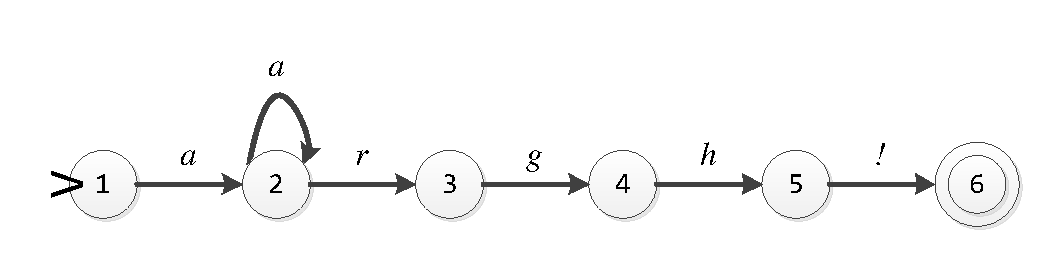
\includegraphics[scale=0.8]{screaming_machine}
	\end{figure}
	

\end{frame}



\begin{frame}

	\frametitle{\insertsection}
	\framesubtitle{\insertsubsection}
	
	
	\begin{itemize}
		\item A formal language is a set of strings.
		\item The language recognized by an FSM is the set of all strings it recognizes when used in recognition mode.
		\item The language generated by an FSM is the set of all strings it can generate when used in generation mode.
		\item The language accepted and the language generated by an FSM are exactly the same.
	\end{itemize}


\end{frame}


\subsection{Some Examples}

\begin{frame}

	\frametitle{\insertsection}
	\framesubtitle{\insertsubsection}
	
	\only<1>{
		Automaton with a jump arc.
		\begin{figure}
			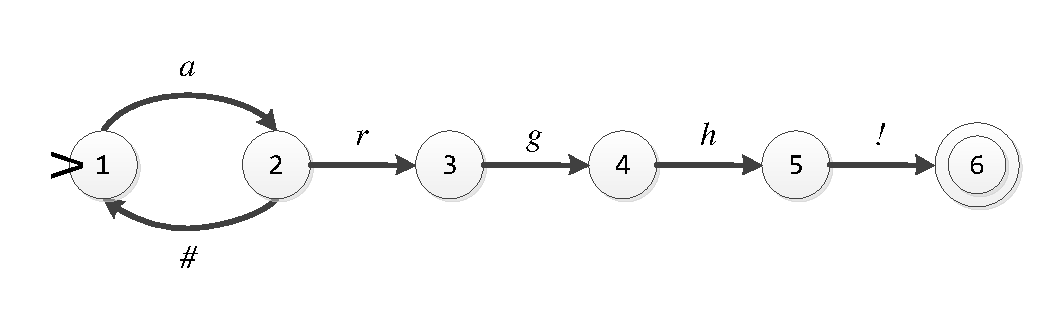
\includegraphics[scale=0.8]{screaming_machine_with_jumps}
		\end{figure}
	}

	\only<2>{
		Another alphabet.
		\begin{figure}
			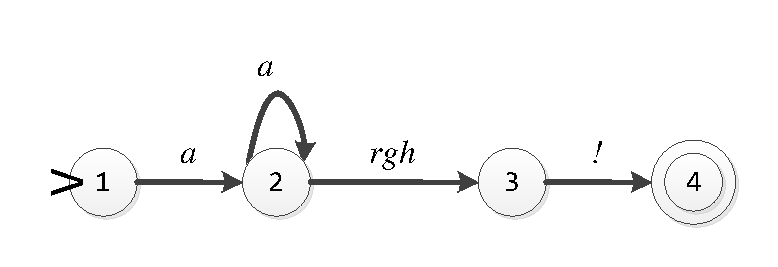
\includegraphics[scale=0.85]{complex_alphabet}
		\end{figure}
	}

	\only<3->{
		Automaton with multiple final states.
		\begin{figure}
			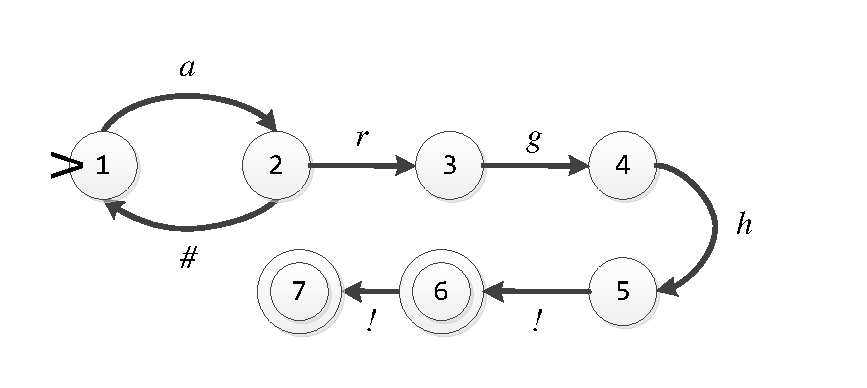
\includegraphics[scale=0.85]{multiple_finals}
		\end{figure}
	}


\end{frame}


\subsection{Deterministic and Non-deterministic Automata}


\begin{frame}

	\frametitle{\insertsection}
	\framesubtitle{\insertsubsection}
	
	
	\begin{figure}
		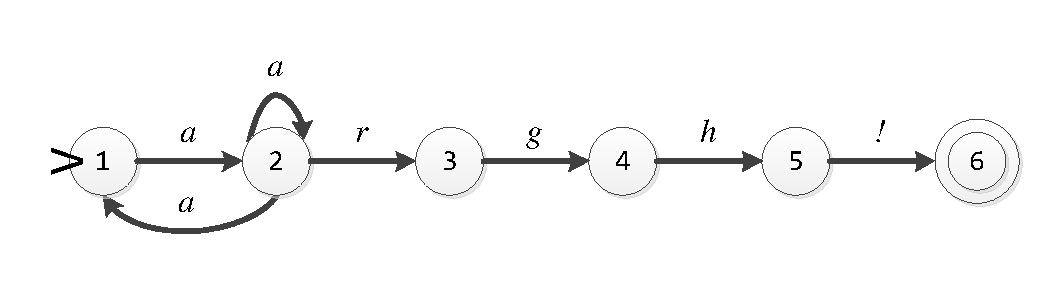
\includegraphics[scale=0.8]{nondet}
	\end{figure}


\end{frame}


\begin{frame}

	\frametitle{\insertsection}
	\framesubtitle{\insertsubsection}
	
	\begin{itemize}
		\item This automaton has two arcs labelled with the same symbol going out of one state -- this FSA is \textbf{non-deterministic}.
		\item Non-determinism doesn't add anything to what FSAs can do.
		\item When using an automaton for generation, there is no big difference between deterministic and non-deterministic machines.
		\item There is, however, a difference when we want to use the machine for recognition: non-determinism brings with it the need to perform \textbf{search}.
	\end{itemize}

\end{frame}


\subsection{Implementing FSA in Prolog}


\begin{frame}

	\frametitle{\insertsection}
	\framesubtitle{\insertsubsection}
	
	\begin{itemize}
		\item We are going to treat FSAs as passive data structures that are manipulated by other programs.
		\item Separating declarative and procedural information is often a good idea.
		\item We will use three predicates to represent FSAs:
		\texttt{\begin{enumerate}
			\item start/1
			\item end/1
			\item arc/3
		\end{enumerate}}
	\end{itemize}

\end{frame}


\begin{frame}

	\frametitle{\insertsection}
	\framesubtitle{\insertsubsection}
	
	\only<1>{
		Simple screaming machine
		\texttt{\begin{itemize}
			\item[] start(1).
			\item[] end(6).
			\item[] arc(1,2,a).
			\item[] arc(2,3,r).
			\item[] arc(2,2,a).
			\item[] arc(3,4,g).
			\item[] arc(4,5,h).
			\item[] arc(5,6,!).
	\end{itemize}}}

	\only<2>{
		Non-deterministic screaming machine
		\texttt{\begin{itemize}
				\item[] start(1).
				\item[] end(6).
				\item[] arc(1,2,a).
				\item[] arc(2,3,r).
				\item[] arc(2,1,a).
				\item[] arc(2,2,a).
				\item[] arc(3,4,g).
				\item[] arc(4,5,h).
				\item[] arc(5,6,!).
	\end{itemize}}}

	\only<3->{
		Screaming machine with a jumping arc
		\texttt{\begin{itemize}
				\item[] start(1).
				\item[] end(6).
				\item[] arc(1,2,a).
				\item[] arc(2,3,r).
				\item[] arc(2,1,'\#').
				\item[] arc(3,4,g).
				\item[] arc(4,5,h).
				\item[] arc(5,6,!).
	\end{itemize}}}

\end{frame}


\begin{frame}

	\frametitle{\insertsection}
	\framesubtitle{\insertsubsection}
	
	\only<1>{
		\textbf{Recognizer and Generator without jump arcs}
		\texttt{\begin{itemize}
				\item[] recognize(Node,[]) :- end(Node).
				\item[] recognize(Node,String) :- arc(Node,Next,Label), \\ \quad\quad\quad\quad\quad\quad\quad\quad\quad\quad\quad\quad traverse(Label,String,NewStr), \\ \quad\quad\quad\quad\quad\quad\quad\quad\quad\quad\quad\quad recognize(Next,NewStr).
				\item[] traverse(Label,[Label|Symbols],Symbols).
				\item[] run(Symbols) :- start(Node),recognize(Node,Symbols).
	\end{itemize}}}

	\only<2->{
		\textbf{Recognizer and Generator with jump arcs}
		\texttt{\begin{itemize}
				\item[] recognize1(Node,[]) :- end(Node).
				\item[] recognize1(Node,String) :- arc(Node,Next,Label), \\ \quad\quad\quad\quad\quad\quad\quad\quad\quad\quad\quad\quad
				traverse1(Label,String,NewStr), \\ \quad\quad\quad\quad\quad\quad\quad\quad\quad\quad\quad\quad
				recognize1(Next,NewStr).
				\item[] traverse1('\#',String,String).
				\item[] traverse1(Label,[Label|Symbols],Symbols).
				\item[] run1(Symbols) :- start(Node),recognize1(Node,Symbols).
	\end{itemize}}}

\end{frame}


\subsection{Finite State Methods in Computational Linguistics and NLP}


\begin{frame}

	\frametitle{\insertsection}
	\framesubtitle{\insertsubsection}
	
	\begin{itemize}
		\item Finite state machines are very simple, but there are limitations to what they can do.
		\item FSA can only recognize and generate \textbf{Regular Languages}.
		\item Many linguistic phenomena can only be described by languages which cannot be generated by FSAs.
		\item There are, however, linguistic applications where the expressive power of finite state methods seems to be sufficient.
		\item Finite state methods have been shown to be particularly useful in the areas of phonological and morphological processing, and have also been applied to syntactic analysis.
	\end{itemize}

\end{frame}


\section{Finite State Parsers and Transducers}

\begin{frame}

	\begin{center}
		\Huge \insertsection
	\end{center}

\end{frame}


\begin{frame}

	\frametitle{\insertsection}
	
	\begin{enumerate}
	\item Building Structure while Recognizing
	\begin{enumerate}
		\item Finite State Parsers
		\item Separating out the Lexicon
	\end{enumerate}
	\item Finite State Transducers
	\begin{enumerate}
		\item What are Finite State Transducers?
		\item FSTs in Prolog
	\end{enumerate}
	\item Morphological Analysis with Finite State Transducers
	\end{enumerate}

\end{frame}

\subsection{Building Structure while Recognizing}

\begin{frame}

	\frametitle{\insertsection}
	\framesubtitle{\insertsubsection}
	
	\begin{itemize}
		\item In addition to knowing that something is accepted by a certain FSA, we would like to have an explanation of why it was accepted.
		\item \textbf{Finite State Parsers} give us that kind of explanation by returning the sequence of transitions that was made.
		\item The parser output should tell us about the transitions that had to be made in the FSA when the input was recognized.
		\item There is a standard technique in Prolog for turning a recognizer into a parser: add one or more extra arguments to keep track of the structure that was found.
	\end{itemize}

\end{frame}


\begin{frame}

	\frametitle{\insertsection}
	\framesubtitle{\insertsubsection}
	
	In the base clause, when the input is read and the FSA is in a final state, all we have to do is record that final state.
	
	\uncover<1->{
		\texttt{\begin{itemize}
				\item[] recognize(Node,[]) :- end(Node).
		\end{itemize}}
	}

	\uncover<2->{
		\texttt{\begin{itemize}
				\item[] parse(Node,[Node],[]) :- end(Node).
		\end{itemize}}
	}

\end{frame}


\begin{frame}

	\frametitle{\insertsection}
	\framesubtitle{\insertsubsection}
	
	The recursive clause looked as follows:
	
	\uncover<1->{
		\texttt{\begin{itemize}
				\item[] recognize(Node,String) :- arc(Node,Next,Label),\\ \quad\quad\quad\quad\quad\quad\quad\quad\quad\quad\quad\quad
				traverse(Label,String,NewStr),\\ \quad\quad\quad\quad\quad\quad\quad\quad\quad\quad\quad\quad
				recognize(Next,NewStr).
		\end{itemize}}
	}
	
	\uncover<2->{
		\texttt{\begin{itemize}
				\item[] parse(Node,[Node,Label|Path],String) :- arc(Node,Next,Label), \\ \quad\quad\quad\quad\quad\quad\quad\quad\quad\quad\quad\quad
				traverse(Label,String,NewStr), \\ \quad\quad\quad\quad\quad\quad\quad\quad\quad\quad\quad\quad
				parse(Next,Path,NewStr).
		\end{itemize}}
	}

\end{frame}


\begin{frame}

	\frametitle{\insertsection}
	\framesubtitle{\insertsubsection}
	
	Finally the whole program looks like this:
	
	\texttt{\begin{itemize}
			\item[] parse(Node,[Node],[]) :- end(Node).
			\item[] parse(Node,[Node,Label|Path],String) :- arc(Node,Next,Label), \\ \quad\quad\quad\quad\quad\quad\quad\quad\quad\quad\quad\quad
			traverse(Label,String,NewStr), \\ \quad\quad\quad\quad\quad\quad\quad\quad\quad\quad\quad\quad
			parse(Next,Path,NewStr).
			\item[] runParser(Symbols,Structure) :- start(Node), \\ \quad\quad\quad\quad\quad\quad\quad\quad\quad\quad\quad\quad
			parse(Node,Structure,Symbols), \\ \quad\quad\quad\quad\quad\quad\quad\quad\quad\quad\quad\quad
			atomics\_to\_string(Structure,' ',Out), \\ \quad\quad\quad\quad\quad\quad\quad\quad\quad\quad\quad\quad
			writeln(Out).
	\end{itemize}}

\end{frame}


\begin{frame}

	\frametitle{\insertsection}
	\framesubtitle{\insertsubsection}
	
	\begin{itemize}
		\item The parser records the state the FSA is in and the symbol it is reading on the transition it is taking from this state.
		\item The rest of the path will be specified in the recursive call of \texttt{parse/3} and collected in the variable \texttt{Path}.
		\item Calling \texttt{runParser(\_,\_)} we will get all possible screams along with a full information about how exactly these words were generated.
	\end{itemize}

\end{frame}


\begin{frame}

	\frametitle{\insertsection}
	\framesubtitle{\insertsubsection}
	
	Let us have a look at the FSA below:
	
	\begin{figure}
		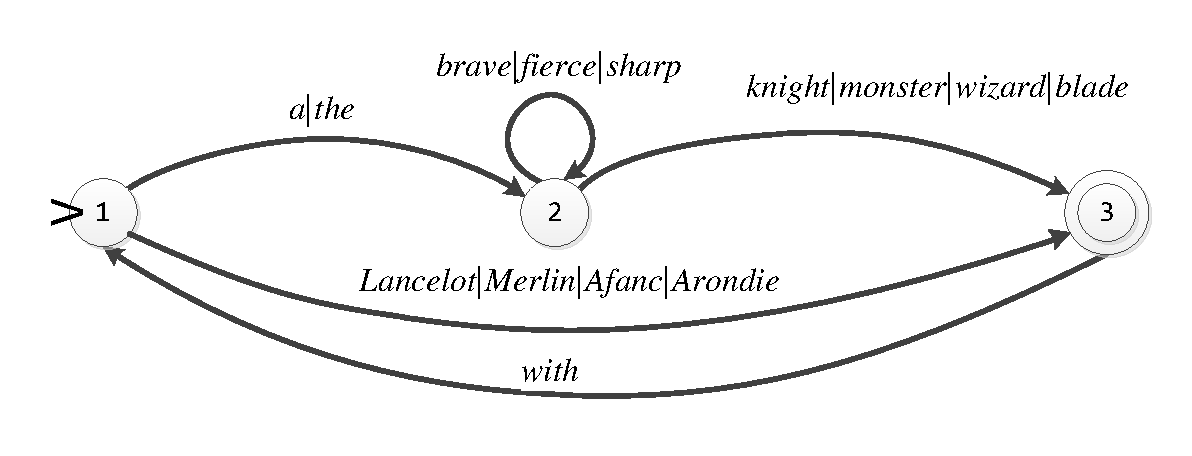
\includegraphics[scale=0.7]{myphology}
	\end{figure}


\end{frame}


\begin{frame}

	\frametitle{\insertsection}
	\framesubtitle{\insertsubsection}
	
	If you decided to construct it with Prolog you would probably end up with something like this:
	
	\texttt{\begin{table}
		\centering
		\begin{tabular}{ l | r }
			\rowcolor{LightGray} start(1). & arc(1,3,merlin). \\
			\rowcolor{LightGray} end(3). & arc(1,3,afanc). \\
			\rowcolor{LightGray} arc(1,2,a). & arc(1,3,arondie). \\
			\rowcolor{LightGray} arc(1,2,the). & arc(2,3,knight). \\
			\rowcolor{LightGray} arc(2,2,brave). & arc(2,3,monster). \\
			\rowcolor{LightGray} arc(2,2,fierce). & arc(2,3,wizard). \\
			\rowcolor{LightGray} arc(2,2,sharp). & arc(2,3,blade). \\
			\rowcolor{LightGray} arc(1,3,lancelot). &  arc(3,1,with).
		\end{tabular}
	\end{table}}

\end{frame}


\begin{frame}

	\frametitle{\insertsection}
	\framesubtitle{\insertsubsection}
	
	\begin{itemize}
		\item If we used the parser of the previous section on this automaton to parse the input \texttt{[a,knight,with,a,blade]}, it would return (\texttt{1 a 2 knight 3 with 1 a 2 blade 3}).
		\item But in a way, it would be even nicer, if we got a more abstract explanation saying, e.g., that \texttt{[a,knight,with,a,blade]} is a noun phrase because it consists of a determiner followed by an noun which is followed by an another noun phrase.
		\item (\texttt{1 det 2 common noun 3 prep 1 det 2 common noun 3}).
		\item In fact, it would be a lot nicer, if you could specify transitions in the FSA based on \textbf{categories} like determiner, common noun, and so on and additionally give a separate lexicon which specifies what words belong to a category.
	\end{itemize}


\end{frame}


\begin{frame}

	\frametitle{\insertsection}
	\framesubtitle{\insertsubsection}
	
	Like this, for example:
	
	\texttt{\begin{table}
			\centering
			\begin{tabular}{ l | r | r }
				\rowcolor{LightGray} start(1). & lex(a, det). & lex(wizard,cn).\\
				\rowcolor{LightGray} end(3). & lex(the,det). & lex(blade,cn).\\
				\rowcolor{LightGray} arc(1,2,det). & lex(fast,adj). & lex(lancelot,pn).\\
				\rowcolor{LightGray} arc(2,2,adj). & lex(fierce,adj). & lex(merlin,pn).\\
				\rowcolor{LightGray} arc(2,3,cn). & lex(sharp,adj). & lex(aranc,pn).\\
				\rowcolor{LightGray} arc(1,3,pn). & lex(knight,cn). & lex(arondie,pn).\\
				\rowcolor{LightGray} arc(3,1,prep. & lex(monster,cn). & lex(with,prep).\\
			\end{tabular}
	\end{table}}

\end{frame}


\begin{frame}

	\frametitle{\insertsection}
	\framesubtitle{\insertsubsection}
	
	It's not very difficult to change our recognizer to work with FSA specifications that, like the above, define their transitions in terms of categories instead of symbols and then use a lexicon to map those categories to symbols or the other way round. The only thing that changes is the definition of the \texttt{traverse} predicate. We don't simply compare the label of the arc with the next symbol of the input anymore, but have to access the lexicon to check whether the next symbol of the input is a word of the category specified by the label of the arc.

\end{frame}


\subsection{Finite State Transducers}


\begin{frame}

	\frametitle{\insertsection}
	\framesubtitle{\insertsubsection}
	
	\begin{itemize}
		\item A \textbf{Finite State Transducer} essentially is a \textbf{FSA} that works on two (or more) tapes. They read from one of the tapes and write onto the other.
		\item Transducers can be used in other modes than the translation mode as well: in the generation mode transducers write on both tapes and in the recognition mode they read from both tapes. Furthermore, the direction of translation can be turned around.
	\end{itemize}

\end{frame}


\begin{frame}

	\frametitle{\insertsection}
	\framesubtitle{\insertsubsection}
	
	This is a transducer that translates 0s into 1s (or vice versa):
	
	\begin{figure}
		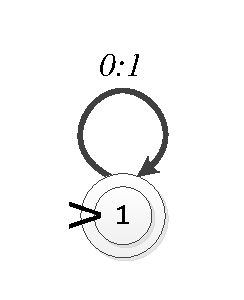
\includegraphics[scale=0.9]{simple_transducer}
	\end{figure}


\end{frame}


\begin{frame}

	\frametitle{\insertsection}
	\framesubtitle{\insertsubsection}
	
	The above transducer behaves as follows in the different modes.
	
	\begin{itemize}
		\item \textbf{Generation mode}: It writes a string of zeros on one tape and a string ones on the other tape. Both strings have the same length.
		\item \textbf{Recognition mode}: It accepts when the word on the first tape consists of exactly as many zeros as the word on the second tape consists of 1s.
		\item \textbf{Translation mode (left to right)}: It reads 0s from the first tape and writes an 1 for every 0 that it reads onto the second tape.
		\item \textbf{Translation mode (right to left)}: It reads 1s from the second tape and writes a 0 for every 1 that it reads onto the first tape.
	\end{itemize}

\end{frame}

\begin{frame}

	\frametitle{\insertsection}
	\framesubtitle{\insertsubsection}
	
	Transitions in transducers can make jumps going from one state to another without doing anything on either one or on both of the tapes. 
	So, transitions of the form 0:\# or \#:0 or \#:\# are possible.
	
	\begin{figure}
		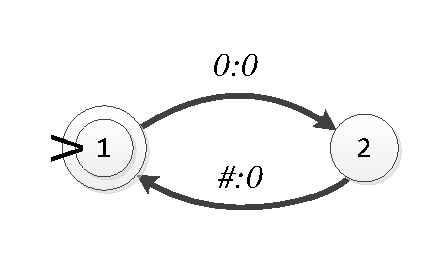
\includegraphics[scale=0.9]{transjump}
	\end{figure}

\end{frame}


\begin{frame}

	\frametitle{\insertsection}
	\framesubtitle{\insertsubsection}
	
	\textbf{What does this transducer do?}
	
	\begin{itemize}
		\item Generation mode: It writes twice as many 0s onto the second tape as onto the first one.
		\item Recognition mode: It accepts when the second tape has twice as many 0s as the first one.
		\item Translation mode (left to right): It reads 0s from the first tape and writes twice as many onto the second tape.
		\item Translation mode (right to left): It reads 0s from the second tape and writes half as many onto the first one.
	\end{itemize}
	
\end{frame}


\begin{frame}

	\frametitle{\insertsection}
	\framesubtitle{\insertsubsection}
	
	In implementing FST in Prolog, we represent it as a static data structure that other programs manipulate.
	Note that to be able to write 0:1 as the label of the arc, we have to define colon as an infix operator as is done by the operator definition.
	
	\texttt{\begin{itemize}
			\item[] :- op(250,xfx,:).
			\item[] 
			\item[] start(1).
			\item[] end(1).
			\item[] arc(1,1,0:1).
	\end{itemize}}

\end{frame}


\begin{frame}

	\frametitle{\insertsection}
	\framesubtitle{\insertsubsection}
	
	Now, we need a program that can manipulate these data structures and carry out the transduction.
	
	\texttt{\begin{itemize}
			\item[] traverse(S1:S2,[S1|Tape1],Tape1,[S2|Tape2],Tape2).
			\item[] transduce(Node,[],[]) :- end(Node).
			\item[] transduce(N,T1,T2) :- arc(N,Nx,St), \\ \quad\quad\quad\quad\quad\quad\quad\quad\quad\quad\quad traverse(St,T1,NT1,T2,NT2),
			 \\ \quad\quad\quad\quad\quad\quad\quad\quad\quad\quad\quad transduce(Nx,NT1,NT2).
			\item[]
			\item[] run(T1,T2) :- start(N),transduce(N,T1,T2).
	\end{itemize}}	

\end{frame}


\begin{frame}

	\frametitle{\insertsection}
	\framesubtitle{\insertsubsection}
	
	Executing program with the first, second or both parameters undefined we can run the transducer in various modes.
	
	\begin{figure}
		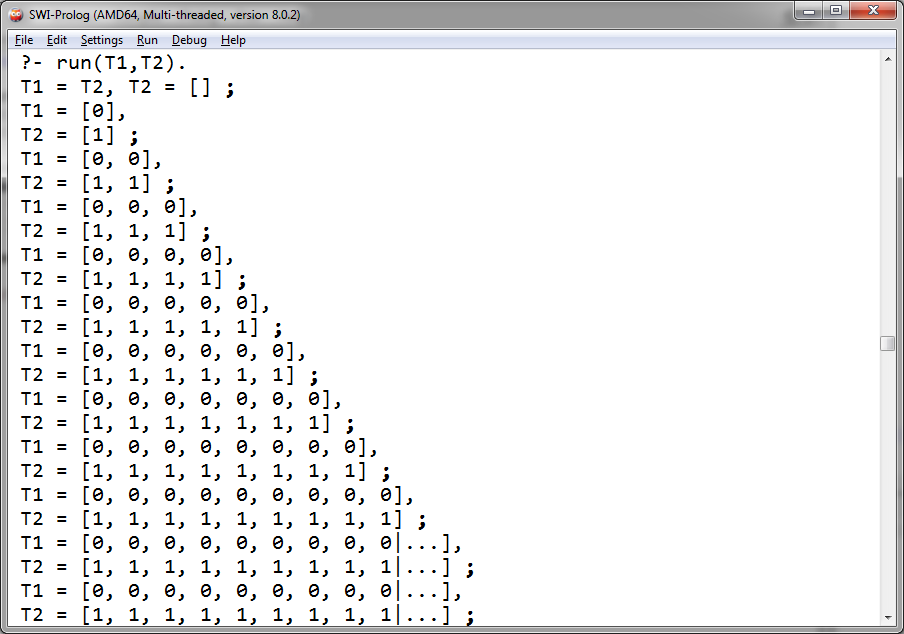
\includegraphics[scale=0.27]{transducer1_screen}
	\end{figure}

\end{frame}

\begin{frame}

	\frametitle{\insertsection}
	\framesubtitle{\insertsubsection}
	
	To be able to use the second transducer, the zero doubler we need a program that can handle transitions involving jumps.
	The only thing that changes is the way that the tapes are treated when making a transition.
	This is taken care of by the \texttt{traverse1/4} predicate and this is all we have to adapt.
	
	\texttt{\begin{itemize}
			\item[] traverse1('\#':S2,Tape1,Tape1,[S2|Tape2],Tape2).
			\item[] traverse1(S1:S2,[S1|Tape1],Tape1,[S2|Tape2],Tape2).
	\end{itemize}}	

\end{frame}


\begin{frame}

\frametitle{\insertsection}
\framesubtitle{\insertsubsection}

	And this is how it works.
	
	\begin{figure}
		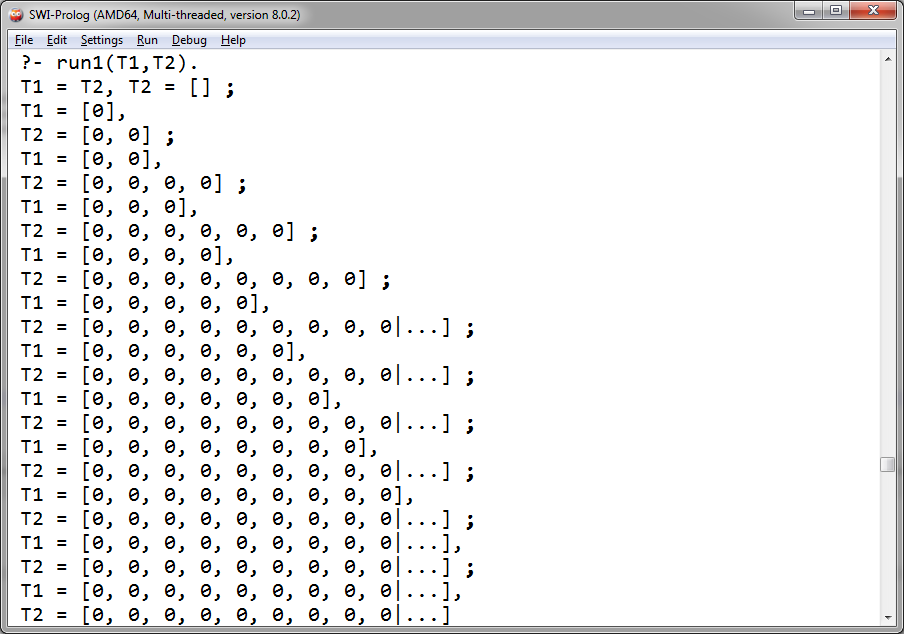
\includegraphics[scale=0.27]{transducer2_screen}
	\end{figure}

\end{frame}


\subsection{Morphological Analysis with Finite State Transducers}


\begin{frame}

	\frametitle{\insertsection}
	\framesubtitle{\insertsubsection}
	
	\begin{itemize}
		\item Morphology is about the internal structure of words.
		\item It asks of what are the building blocks -- the morphemes -- that a word is constructed from and what is the meaning of these blocks.
		 And what are the rules by which these building blocks can be combined to form words?
		\item For instance the word \textit{''share``} consists of one morpheme \textit{share}, while \textit{''shared``} consists of two morphemes, namely
		the \textbf{stem} \textit{share} and the past tense \textit{d}. The word \textit{''blessed``} also consists of two morphemes, but now the past tense
		is \textit{ed}.
		\item Morphology is an area of computational linguistics where finite state technology has been found to be particularly useful, because for many languages the rules after which morphemes can be combined to build words can be caputered by finite state automata.
		\item It is possible to write finite state transducers that map the surface form of a word to a description of the morphemes that constitute that word or vice versa.
	\end{itemize}
	

\end{frame}



\begin{frame}

	\frametitle{\insertsection}
	\framesubtitle{\insertsubsection}
	
	\begin{itemize}
		\item Such transducers could, for instance, map \textit{share+d} and \textit{bless+ed} to \textit{share+PAST} and \textit{bless+PAST} respectively.
		\item As an example we will look at past forms of verbs in English.
		\item The default rule is to add \textit{ed} or \textit{d} to a normal form.
		\item But there also are the irregular verbs, such as \textit{run}, \textit{teach}, \textit{think} etc.
	\end{itemize}

\end{frame}


\begin{frame}

	\frametitle{\insertsection}
	\framesubtitle{\insertsubsection}
	
	We want a transducer that would translate \textit{shared} to \textit{share-PAST}, \textit{blessed} to \textit{bless-PAST}, \textit{thought} to \textit{think-PAST} and so on.
	
	\begin{figure}
		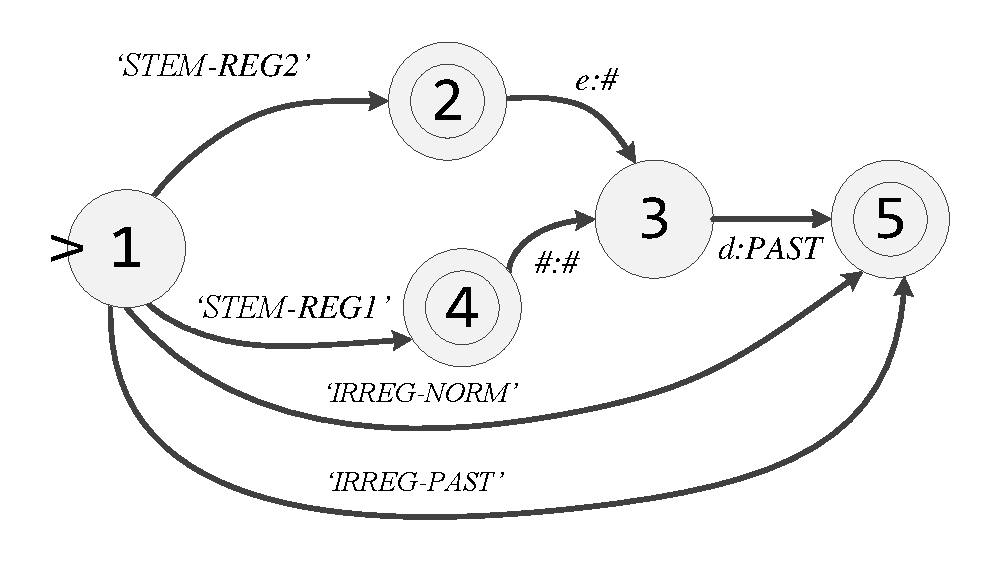
\includegraphics[scale=0.67]{morphtransducer}
	\end{figure}

\end{frame}


\begin{frame}

	\frametitle{\insertsection}
	\framesubtitle{\insertsubsection}
	
	As before, we split our lexicon into categories.
	
	\texttt{\begin{itemize}
			\item[] lex(bless:bless, 'STEM-REG2').
			\item[] lex(share:share, 'STEM-REG1').
			\item[] lex(run:run, 'IRREG-NORM').
			\item[] lex(think:think, 'IRREG-NORM').
			\item[] lex(ran:'run-PAST', 'IRREG-PAST').
			\item[] lex(thought:'think-PAST', 'IRREG-PAST').
			\item[] \ldots
	\end{itemize}}

\end{frame}


\begin{frame}

	\frametitle{\insertsection}
	\framesubtitle{\insertsubsection}
	
	\begin{itemize}
		\item The above transducer assumes that the words are already split up into morphemes (such as stem and the past tense suffix).
		\item If it was implemented in Prolog it would assume input of the form \texttt{[share,d]} on the first tape.
		\item In order to be able to input plain strings we should use another transducer that would split the strings for us, and then use these two transducers in a cascade.
		\item That is, we let the morphological transducer run on the output of the splitting transducer, and compose them into a single transducer that performs both tasks.
	\end{itemize}
	
\end{frame}


\section{Finite State Methods in NLP}

\begin{frame}

	\begin{center}
		\Huge \insertsection
	\end{center}

\end{frame}


\begin{frame}

	\frametitle{\insertsection}
	
	\begin{enumerate}
		\item Morphology
		\item Morph parsing
		\item Regular relation and languages
	\end{enumerate}

\end{frame}


\subsection{Morphology}

\begin{frame}

	\frametitle{\insertsection}
	\framesubtitle{\insertsubsection}
	
	\begin{itemize}
		\item Morphology is interested in what are the smallest units in word that bear some meaning and how can they be combined to form words.
		\item The smallest unit in a word that bear some meaning are called \textbf{morphemes}.
		\item Morphemes that contribute the main meaning of a word are called \textbf{stems}, while the other morphemes are known as \textbf{affixes}.
		\item How can morphemes be combined to form words that are legal in some language ?
	\end{itemize}

\end{frame}

\subsection{Morph parsing}

\begin{frame}

	\frametitle{\insertsection}
	\framesubtitle{\insertsubsection}
	
	The goal of \textbf{morphological parsing} is to find out what morphemes a given word is built from.
	
	\begin{table}
			\centering
			\begin{tabular}{ l c l }
				\rowcolor{LightGray} car & car & Noun SG \\
				\rowcolor{LightGray} cars & car & Noun PL \\
				\rowcolor{LightGray} foot & foot & N SG \\
				\rowcolor{LightGray} feet & foot & Noun PL \\
				\rowcolor{LightGray} bosses & boss & N PL \\
			\end{tabular}
	\end{table}

\end{frame}


\begin{frame}

	\frametitle{\insertsection}
	\framesubtitle{\insertsubsection}
	
	Morphological parsing yields information that, for instance helps to know the agreement features of words.
	Grammar checkers need to know agreement information to detect mistakes. 
	Morphological information also helps spell checkers to decide whether something is a possible word or not, 
	and in information retrieval it is used to search not only one form of a word, but also all other possible forms.

\end{frame}


\begin{frame}

	\frametitle{\insertsection}
	\framesubtitle{\insertsubsection}
	
	To get morphological information about a word, given it's surface form, we need to proceed in some steps.
	
	\begin{itemize}
		\item Split a word up into it's possible components and indicate morpheme boundaries. For example, we are going to make \textit{car+s} out of \textit{cars}.
		There may be multiple ways of splitting up a word.
		\item Use a lexicon of stems to look up the categories of the stems and the meaning of the affixes. So \textit{boss+s} will be mapped
		to \textit{boss~Noun~PL}, and \textit{feet} to \textit{foot~Noun~PL}.
	\end{itemize}

\end{frame}



\begin{frame}

	\frametitle{\insertsection}
	\framesubtitle{\insertsubsection}
	
	\begin{table}
		\centering
		\begin{tabular}{ l | c | l }
			\rowcolor{Gray}
			\textbf{Surface form} & \textbf{Intermediate form} & \textbf{Morphological Structure} \\
			\rowcolor{LightGray} car & car & car Noun SG \\
			\rowcolor{LightGray} cars & car+s & car Noun PL \\
			\rowcolor{LightGray} foot & foot & foot N SG \\
			\rowcolor{LightGray} feet & feet & foot Noun PL \\
			\rowcolor{LightGray} bosses & boss+s & boss N PL \\
		\end{tabular}
	\end{table}

\end{frame}


\begin{frame}

	\frametitle{\insertsection}
	\framesubtitle{\insertsubsection}
	
	From the surface form to the intermediate form.
	
	\begin{figure}
		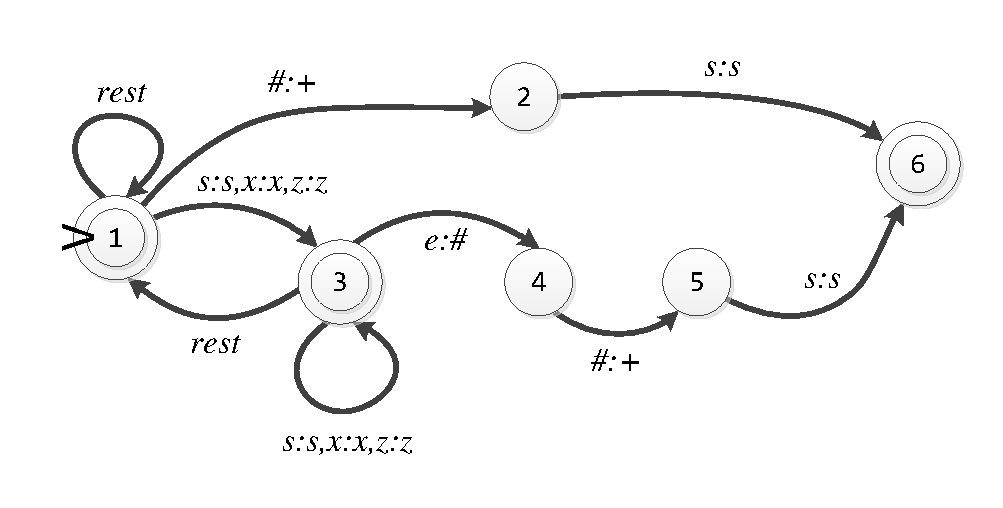
\includegraphics[scale=0.67]{surface2imf}
	\end{figure}

\end{frame}



\begin{frame}

	\frametitle{\insertsection}
	\framesubtitle{\insertsubsection}
	
	From the Intermediate Form to the Morphological Structure.
	
	The input that this transducer has to accept is of one of the following:
	
	\begin{enumerate}
		\item Regular noun stem (\textit{car, boss, etc.}). Map all symbols of the stem to themselves and then output \textbf{N} and \textbf{SG}.
		\item Regular noun stem + s (\textit{car+s, boss+s, etc.}). Map all symbols of the stem to themselves, and then output \textbf{N} and replace \textbf{s} with \textbf{PL}.
		\item Singular irregular noun stem (\textit{foot, woman, etc.}). Do the same as in the first case.
		\item Plural irregular noun stem (\textit{feet}). Map the irregular plural noun stem to the corresponding singular stem, and then add \textbf{N} and \textbf{PL}.
	\end{enumerate}

\end{frame}


\begin{frame}

	\frametitle{\insertsection}
	\framesubtitle{\insertsubsection}
	
	From the Intermediate Form to the Morphological Structure.
	
	\begin{figure}
		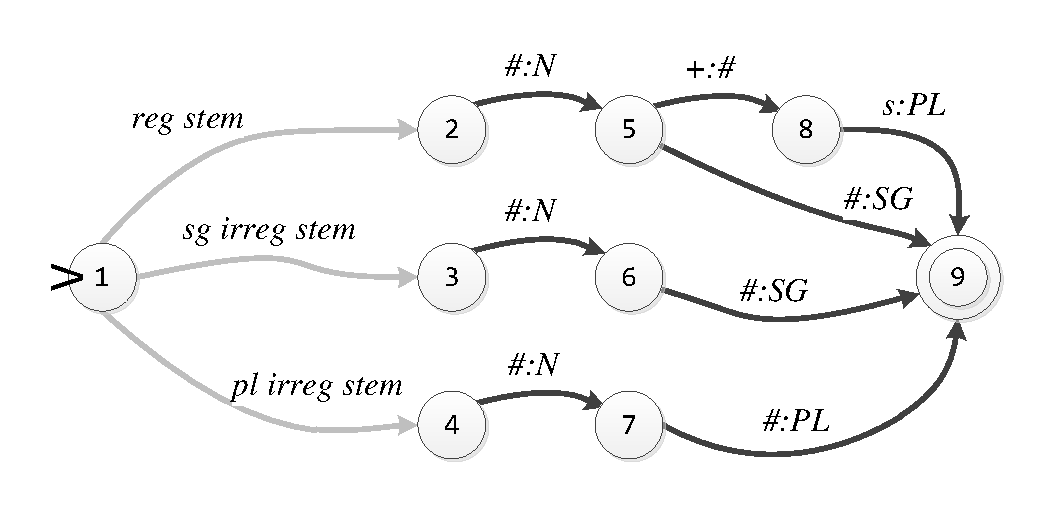
\includegraphics[scale=0.67]{imf2udl}
	\end{figure}

\end{frame}


\begin{frame}

	\frametitle{\insertsection}
	\framesubtitle{\insertsubsection}
	
	\begin{itemize}
		\item What still needs to be specified is how exactly the parts between state 1 and states 2,3, and 4 respectively look like.
		\item We need to recognize noun stems and decide whether they are regular or not.
		\item it is done by encoding a lexicon.
	\end{itemize}
	
	\begin{figure}
		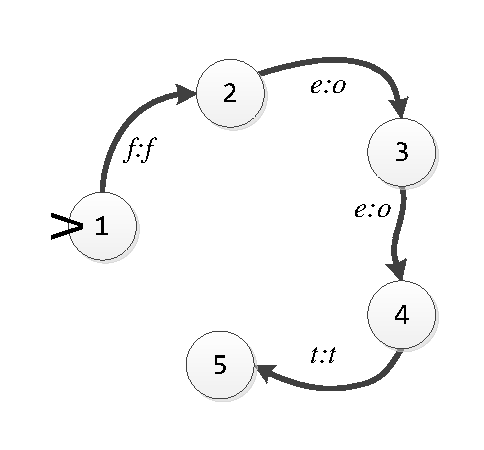
\includegraphics[scale=0.67]{feet2foot}
	\end{figure}

\end{frame}


\begin{frame}

	\frametitle{\insertsection}
	\framesubtitle{\insertsubsection}
	
	\begin{itemize}
		\item If we let the two transducers run in a cascade, we can do a morphological parse of (some) English noun phrases.
		\item We can also use this transducer for generating a surface form from an underlying form.
		\item There are algorithms for combining several cascaded tranducers or multiple transducers that are supposed to be applied in parallel into a single transducer. However, these algorithms only work, if the individual transducers obey some restrictions so that some care has to be taken when specifying them.
	\end{itemize}
	
\end{frame}


\subsection{Regular relations and languages}


\begin{frame}

	\frametitle{\insertsection}
	\framesubtitle{\insertsubsection}
	
	\begin{itemize}
		\item As we have seen before, we don't always have to specify one big transducer that can deal with all spelling rules, but that it is enough to specify one small transducer per rule, because there are ways of combining these individual transducers into one big transducer.
		\item Still you might think that specifying the e-insertion transducer was actually quite tricky.
		\item But there is way of formulating spelling rules that makes it possible to automatically translate them into transducers.
	\end{itemize}

\end{frame}


\begin{frame}

	\frametitle{\insertsection}
	\framesubtitle{\insertsubsection}
	
	\begin{itemize}
		\item The languages that FSA can recognize are called \textbf{regular}.
		\item Every Regular Language can be specified with a \textbf{Regular Expression}.
		\begin{enumerate}
			\item Let us have an \textbf{alphabet} \(\Sigma = (c_1,c_2,\ldots,c_k) \). For every \textbf{i} \(c_i\) is a regular expression.
			\item \(\varepsilon \) is a regular expression (an empty word).
			\item If \(\alpha_1 \) and \(\alpha_2 \) are regular expressions then \((\alpha_1 | \alpha_2) \) and \((\alpha_1)(\alpha_2) \) are
			regular expressions.
			\item If \(\alpha \) is a regular expression then \((\alpha)^{*} \) is a regular expression.
		\end{enumerate}
		\item \textbf{There is a systematic way of translating regular expressions into finite state automata.}
	\end{itemize}

\end{frame}


\begin{frame}

	\frametitle{\insertsection}
	\framesubtitle{\insertsubsection}
	
	\begin{itemize}
		\item Finite state transducers recognize tuples of strings.
		\item A set of tuples of strings that can be recognized by an FST is called a \textbf{Regular Relation}.
		\item Languge spelling rules can be specified as regular relations.
		\item There are algorithms for translating such rule systems (at least, as long as they obey certain restrictions) into transducers.
	\end{itemize}

\end{frame}